En este pasaje se habla sobre el diagrama de estados del sistema. El objetivo de este consiste en representar el funcionamiento de la lógica que se encuentra en Node-Red.

Cabe aclarar que por cuestiones de practicidad, en la Imagen (\ref{fig:diagrama_de_estados}) se simbolizan con nodos rojos, la interacción que el usuario tenga con la interfaz gráfica. Estos nodos representan los datos que se ingresan en el servidor por parte del cliente. Es decir, una comunicación unidireccional de la persona hacia el nido.

\begin{figure}[H]
	\centering	
	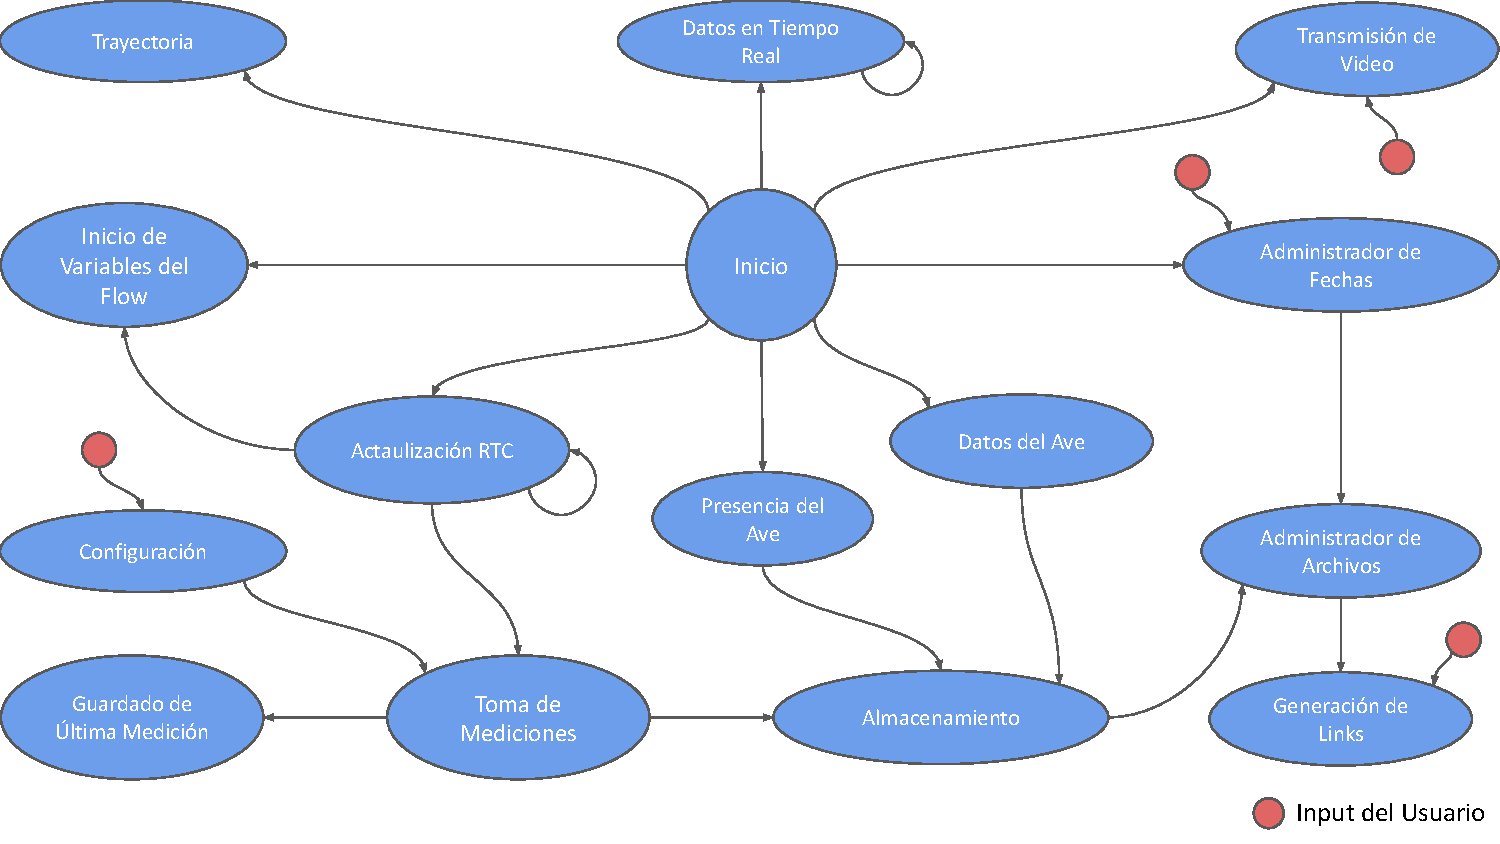
\includegraphics[width=\textwidth, page=1]{ImagenesIngenieria de Detalle/FlowChartNodeRed.pdf}	
	\caption{Diagrama de estados.}
	\label{fig:diagrama_de_estados}
\end{figure}
